% This is "sig-alternate.tex" V2.1 April 2013
% This file should be compiled with V2.5 of "sig-alternate.cls" May 2012
%
% This example file demonstrates the use of the 'sig-alternate.cls'
% V2.5 LaTeX2e document class file. It is for those submitting
% articles to ACM Conference Proceedings WHO DO NOT WISH TO
% STRICTLY ADHERE TO THE SIGS (PUBS-BOARD-ENDORSED) STYLE.
% The 'sig-alternate.cls' file will produce a similar-looking,
% albeit, 'tighter' paper resulting in, invariably, fewer pages.
%
% ----------------------------------------------------------------------------------------------------------------
% This .tex file (and associated .cls V2.5) produces:
%       1) The Permission Statement
%       2) The Conference (location) Info information
%       3) The Copyright Line with ACM data
%       4) NO page numbers
%
% as against the acm_proc_article-sp.cls file which
% DOES NOT produce 1) thru' 3) above.
%
% Using 'sig-alternate.cls' you have control, however, from within
% the source .tex file, over both the CopyrightYear
% (defaulted to 200X) and the ACM Copyright Data
% (defaulted to X-XXXXX-XX-X/XX/XX).
% e.g.
% \CopyrightYear{2007} will cause 2007 to appear in the copyright line.
% \crdata{0-12345-67-8/90/12} will cause 0-12345-67-8/90/12 to appear in the copyright line.
%
% ---------------------------------------------------------------------------------------------------------------
% This .tex source is an example which *does* use
% the .bib file (from which the .bbl file % is produced).
% REMEMBER HOWEVER: After having produced the .bbl file,
% and prior to final submission, you *NEED* to 'insert'
% your .bbl file into your source .tex file so as to provide
% ONE 'self-contained' source file.
%
% ================= IF YOU HAVE QUESTIONS =======================
% Questions regarding the SIGS styles, SIGS policies and
% procedures, Conferences etc. should be sent to
% Adrienne Griscti (griscti@acm.org)
%
% Technical questions _only_ to
% Gerald Murray (murray@hq.acm.org)
% ===============================================================
%
% For tracking purposes - this is V2.0 - May 2012

\documentclass{sig-alternate-05-2015}

\usepackage{hyperref}

\usepackage{lmodern}
%% \usepackage{fourier} % Use the Adobe Utopia font for the document - comment this line to return to the LaTeX default
\usepackage[english]{babel} % English language/hyphenation

\usepackage{graphicx}
%% To recognize filenames with extra dots: foo.bar.jpg.
\usepackage{grffile}
\usepackage{algorithmicx}
\usepackage{algpseudocode}
\usepackage{float}
\usepackage{subcaption}

% \usepackage{lipsum} % Used for inserting dummy 'Lorem ipsum' text into the template

% \usepackage{sectsty} % Allows customizing section commands
%% \allsectionsfont{\centering \normalfont\scshape} % Make all sections centered, the default font and small caps

%% For code
\usepackage{listings}
\usepackage{verbatim}

\usepackage{enumitem}
\usepackage{hyperref}
\usepackage{xcolor}
\hypersetup{
  colorlinks,
  linkcolor={red!50!black},
  citecolor={blue!50!black},
  urlcolor={blue!80!black}
}

\begin{document}

% Copyright
\setcopyright{acmcopyright}
%\setcopyright{acmlicensed}
%\setcopyright{rightsretained}
%\setcopyright{usgov}
%\setcopyright{usgovmixed}
%\setcopyright{cagov}
%\setcopyright{cagovmixed}


% DOI
\doi{10.475/123_4}

% ISBN
\isbn{123-4567-24-567/08/06}

%Conference
%% \conferenceinfo{PLDI '13}{June 16--19, 2013, Seattle, WA, USA}

\acmPrice{\$15.00}

%
% --- Author Metadata here ---
%% \conferenceinfo{WOODSTOCK}{'97 El Paso, Texas USA}
%\CopyrightYear{2007} % Allows default copyright year (20XX) to be over-ridden - IF NEED BE.
%\crdata{0-12345-67-8/90/01}  % Allows default copyright data (0-89791-88-6/97/05) to be over-ridden - IF NEED BE.
% --- End of Author Metadata ---

\title{Classification of Reddit Text Posts}
%% \subtitle{[Extended Abstract]
%% \titlenote{A full version of this paper is available as
%% \textit{Author's Guide to Preparing ACM SIG Proceedings Using
%% \LaTeX$2_\epsilon$\ and BibTeX} at
%% \texttt{www.acm.org/eaddress.htm}}}
%
% You need the command \numberofauthors to handle the 'placement
% and alignment' of the authors beneath the title.
%
% For aesthetic reasons, we recommend 'three authors at a time'
% i.e. three 'name/affiliation blocks' be placed beneath the title.
%
% NOTE: You are NOT restricted in how many 'rows' of
% "name/affiliations" may appear. We just ask that you restrict
% the number of 'columns' to three.
%
% Because of the available 'opening page real-estate'
% we ask you to refrain from putting more than six authors
% (two rows with three columns) beneath the article title.
% More than six makes the first-page appear very cluttered indeed.
%
% Use the \alignauthor commands to handle the names
% and affiliations for an 'aesthetic maximum' of six authors.
% Add names, affiliations, addresses for
% the seventh etc. author(s) as the argument for the
% \additionalauthors command.
% These 'additional authors' will be output/set for you
% without further effort on your part as the last section in
% the body of your article BEFORE References or any Appendices.

\numberofauthors{2} %  in this sample file, there are a *total*
% of EIGHT authors. SIX appear on the 'first-page' (for formatting
% reasons) and the remaining two appear in the \additionalauthors section.
%
\author{
% You can go ahead and credit any number of authors here,
% e.g. one 'row of three' or two rows (consisting of one row of three
% and a second row of one, two or three).
%
% The command \alignauthor (no curly braces needed) should
% precede each author name, affiliation/snail-mail address and
% e-mail address. Additionally, tag each line of
% affiliation/address with \affaddr, and tag the
% e-mail address with \email.
%
% 1st. author
\alignauthor
Pradeep Kumar Srinivasan\\
\affaddr{Purdue University}\\
\email{sriniv68@purdue.edu}
% 2nd. author
\alignauthor
Mohammad Haseeb\\
\affaddr{Purdue University}\\
\email{mhaseeb@purdue.edu}
}
% There's nothing stopping you putting the seventh, eighth, etc.
% author on the opening page (as the 'third row') but we ask,
% for aesthetic reasons that you place these 'additional authors'
% in the \additional authors block, viz.
\date{\today}
% Just remember to make sure that the TOTAL number of authors
% is the number that will appear on the first page PLUS the
% number that will appear in the \additionalauthors section.

\maketitle
\begin{abstract}

In this project, we worked on the problem of large text classification, specifically the Reddit Self-Post Classification Task (RSPCT). RSPCT is a dataset with around 1000 classes (``subreddits'') with around 1000 examples per class, which is unique because most text classification datasets have sparse labels. We used two traditional machine learning algorithms and one deep learning algorithm to learn to predict the class (i.e., the subreddit) given the title and body of a post. We evaluated the performance of each model using the Precision-at-K \cite{krizhevsky2012imagenet} metric. We conducted additional experiments like adding features for sentiment analysis and readability level of a post's text \cite{readability} to see if that increases the performance of our models.

\end{abstract}

%
%  Use this command to print the description
%
\printccsdesc

% We no longer use \terms command
%\terms{Theory}

\keywords{NLP; large text classification; multi-class classification}

\section{Introduction}

Text classification with few classes, such as in sentiment analysis, has been well-studied \cite{sentiment-analysis} with state-of-the-art techniques like LSTM. However, those techniques do not always work as well in scenarios with many classes \cite{many-classes}. Another issue with training on many-class datasets is that they have a very large number of labels (such as WikiLSHTC-325K dataset \cite{partalas2015lshtc}, which has 325K labels) and are sparse - most labels in the above dataset have less than 100 examples \cite{jonesreddit}.

We aim to study this problem by using a dataset that has a large number of classes but also a large number of examples per class. To this end, we used the Reddit Self-Post Classification Task (RSPCT) dataset and trained three models and evaluated their performance.

We think this is a useful problem to solve because it has not been adequately studied, to the best of our knowledge, and because this could pave the way to future work on such many-class datasets.

\section{Dataset}

Reddit is a popular social link aggregation, web content rating, and discussion website. Reddit's users submit posts, which are then voted up or down by other members. This allows the highest rated posts to gain the most attention. Reddit is organized into "subreddits", which are sub-forums on Reddit dedicated to a specific topic, for example r/geography, r/gameofthrones, r/MachineLearning.

There are two main types of posts a user can submit on Reddit: a simple URL link and a self-post. A self-post consists of a topic and a body of text and is generally much longer in length, thereby, providing more information to Redditors. Moreover, most of the self-posts talk closely about the subreddit that they were posted in, which makes for a good classification task.

We obtained the Reddit Self-Post Classification Task (RSPCT) dataset from Kaggle \cite{kaggle:dataset}. It is a text corpus containing self-posts (i.e., text posts) from Reddit. RSPCT was collected to help spur research on models that could tackle a large number of classes by ensuring a large population of examples for each class. The data consists of 1.013M self-posts, posted from 1013 subreddits (1000 examples per class). For each post, its title, body and the subreddit that it belongs to are provided.

The aim is to allow for a situation comparable to that in the computer vision community, which was helped by the famous ILSRVC competition (ImageNet \cite{imagenet}) with 1000 classes and around 1400 examples per class. This potential is what made us find this project interesting.

\section{Preprocessing}

As mentioned in the previous section, the RSPCT dataset contains real self-posts from Reddit. This means that the text in these posts may not always conform to the grammar, spelling, vocabulary and other nuances of the English language. For this reason, we carried out a series of preprocessing steps.

Because this is a text classification problem and most of our models used the bag-of-words approach, we first lowercase all the text in the subreddit, title and body of each post. We noticed that many of the posts contained special HTML encoded text and tags like \&gt, \&amp, \&lt, <lb>, <tab> etc. We used regular expression matching to replace these tags with a blank space. We also removed punctuation characters like !, ", \#, \$, \%, \&, (, [, *, + etc. such that we were only left with words at the end of this step.

Finally, we used Python's NLTK's PorterScanner to replace all words with their stem words. This resulted in words like "extremely" and "extreme" to be replaced with "extrem".

\section{Exploratory Data Analysis}

We first explore the dataset by looking at the histogram of the post titles (Figure \ref{fig:sampleLengthDistributionTitle}). We find that most titles are shorter than 100 characters in length, with a median of 35 characters and 7 words.

\begin{figure}[H]
\centering
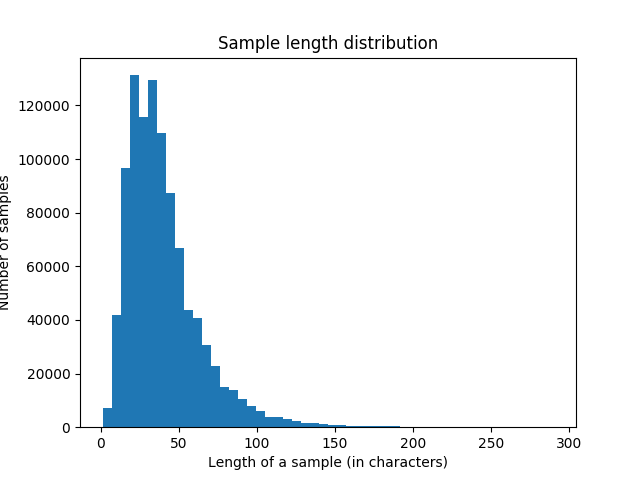
\includegraphics[width=\linewidth]{plots/sample-length-distribution-title-1000000.png}
\caption{Sample Distribution for Length of Post's Title (in characters)}
\label{fig:sampleLengthDistributionTitle}
\end{figure}

Similarly, the histogram for the post bodies (Figure \ref{fig:sampleLengthDistributionSelftext}) shows that most posts are shorter than 1000 characters in length, with a median of 500 characters and 105 words.

\begin{figure}[H]
\centering
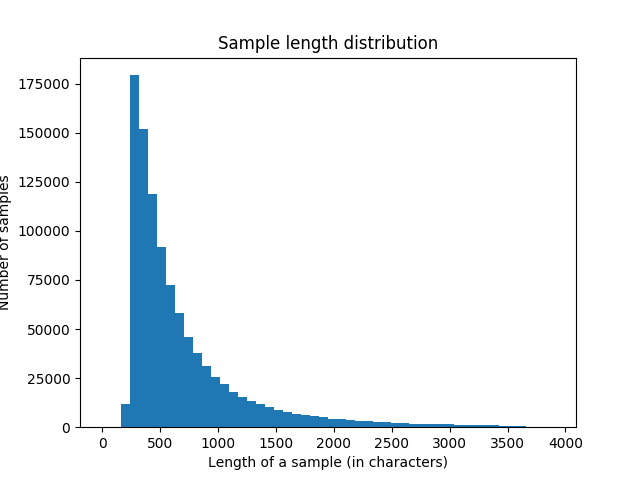
\includegraphics[width=\linewidth]{plots/sample-length-distribution-selftext-1000000.png}
\caption{Sample Distribution for Length of Post's Body (in characters)}
\label{fig:sampleLengthDistributionSelftext}
\end{figure}

The t-SNE\cite{tsne} plot for the subreddits (Figure \ref{fig:tsnePlot}) shows that the subreddits seem to be well-separated by topic. For example, we can see clusters of subreddits for gaming, cryptocurrency, and diseases.

\begin{figure}[H]
\centering
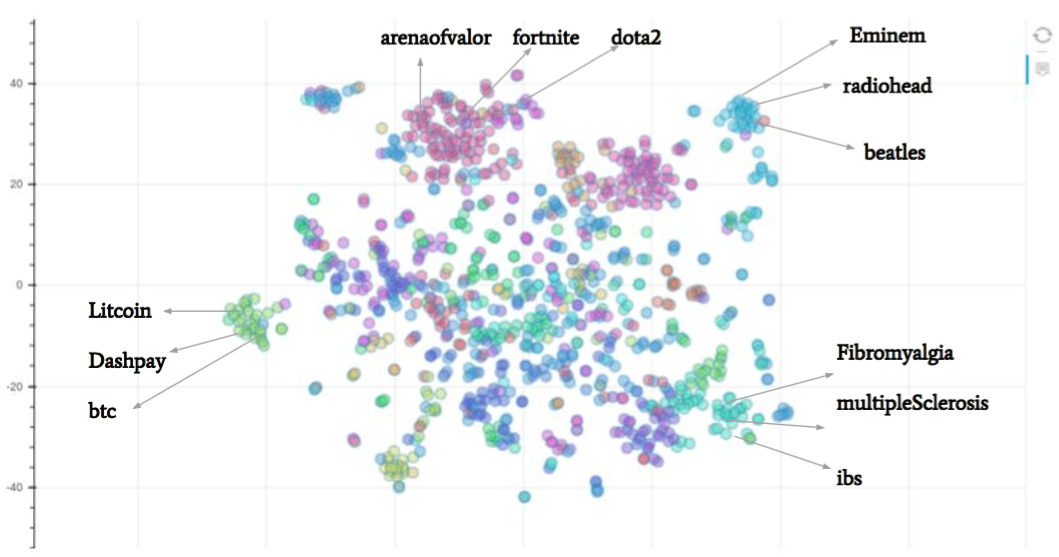
\includegraphics[width=\linewidth]{plots/tsne.png}
\caption{TSNE Plot of All the Self-Posts}
\label{fig:tsnePlot}
\end{figure}

\section{Algorithms Implemented}

\subsection{Data Preparation}

For the two traditional algorithms, we used a label encoder to transform each output label (subreddit name) into a number from 0 to 1012. Then, we used a TF-IDF vectorizer to get 30,000 top words, while excluding stop words and choosing only words that appeared in at least 5 documents and appeared in a maximum of 50\% of the documents. For all three algorithms, we combined the title and body of the posts into one field.

\subsection{Naive Bayes Classifier (NBC)}

The first algorithm we looked at was the Naive Bayes Classifier because of its long use in text classification tasks \cite{rennie2001:improving}. Specifically, we used \verb+MultinomialNB+ from \verb+sklearn+ with the hyperparameter \verb+alpha+.

This model was the fastest to train among the three and gave us a quick baseline with which to compare the others. We also extended the maximum number of feature words to be 100,000 since it did not impact the training time too much. The training curve can be seen in Figure \ref{fig:learningCurveNBC}. We tried the following values of \verb+alpha+: 0.1, 0.5, 0.9, 1.0, and found the best validation accuracy at 0.1.

\begin{figure}[H]
\centering
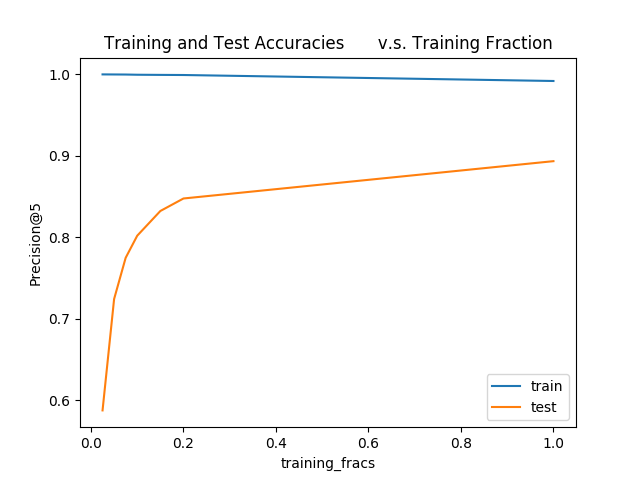
\includegraphics[width=\linewidth]{plots/learning_curve_nbc.png}
\caption{Learning Curve for Naive Bayes Classifier}
\label{fig:learningCurveNBC}
\end{figure}

\subsection{Logistic Regression (LR)}

The next traditional algorithm we wanted to consider was Logistic Regression. We used \verb+LogisticRegression+ from \verb+sklearn.linear_model+ with the hyperparameter C.

The number of feature words used in this bag-of-words \cite{logistic-regression:bag-of-words} approach affected the training time a lot. Similarly, when hyperparameter tuning, we found that while values of C like 0.0001 and 0.01 led to very short training time, they also led to poor validation accuracy. On the other hand, C = 100 (i.e., not penalizing large weight values) led to better validation accuracy but at the cost of orders of magnitude longer training time. The training curve can be seen in Figure \ref{fig:learningCurveLR}.

\begin{figure}[H]
\centering
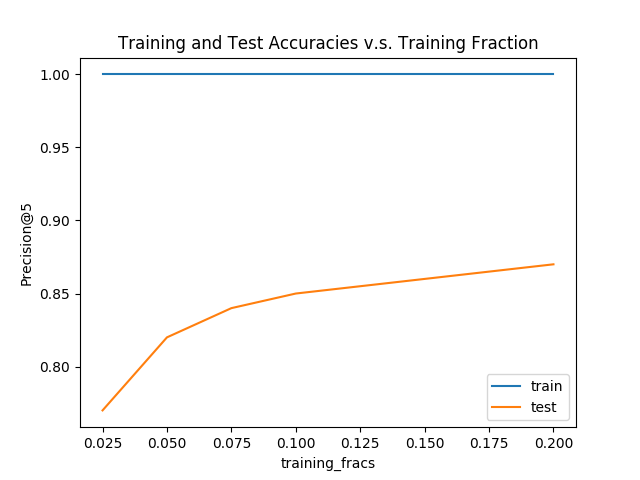
\includegraphics[width=\linewidth]{plots/learning_curve_lr.png}
\caption{Learning Curve for Logistic Regression}
\label{fig:learningCurveLR}
\end{figure}

\subsection{Convolutional Neural Network (CNN)}

Finally, we wanted to test a deep learning model on this dataset. We chose to use a Convolutional Neural Network because of its better average accuracy across different tasks and shorter training time than Recurrent Neural Networks.

To embed the words in the post, we used the GloVe (Global Vectors for Word Representation) embedding \cite{pennington2014glove}. We tried a version with 100 embedding dimensions for each word and another version with 300 embedding dimensions and found the later to give quite a boost in overall accuracy.

We considered two architectures for the CNN, one with three successive layers of filters of size 5 and one with a multi-channel model of filters of sizes 2, 3, and 5. Upon testing, we found that the latter gave much higher accuracy even after a few epochs whereas the former seemed to overfit after a few epochs. So, our multi-channel approach would consider two words at a time, three words at a time, and five words at a time. The later layers use max-pooling and softmax to predict one class label out of 1013 labels. Finally, we use dropout with probability 0.3. The optimizer we use is Adam because of its adaptive learning rate and the loss is categorical cross-entropy.

We trained the CNN for a maximum of 10 epochs over several days and obtained the following learning curve (Figure \ref{fig:learningCurveCNN}).

\begin{figure}[H]
\centering
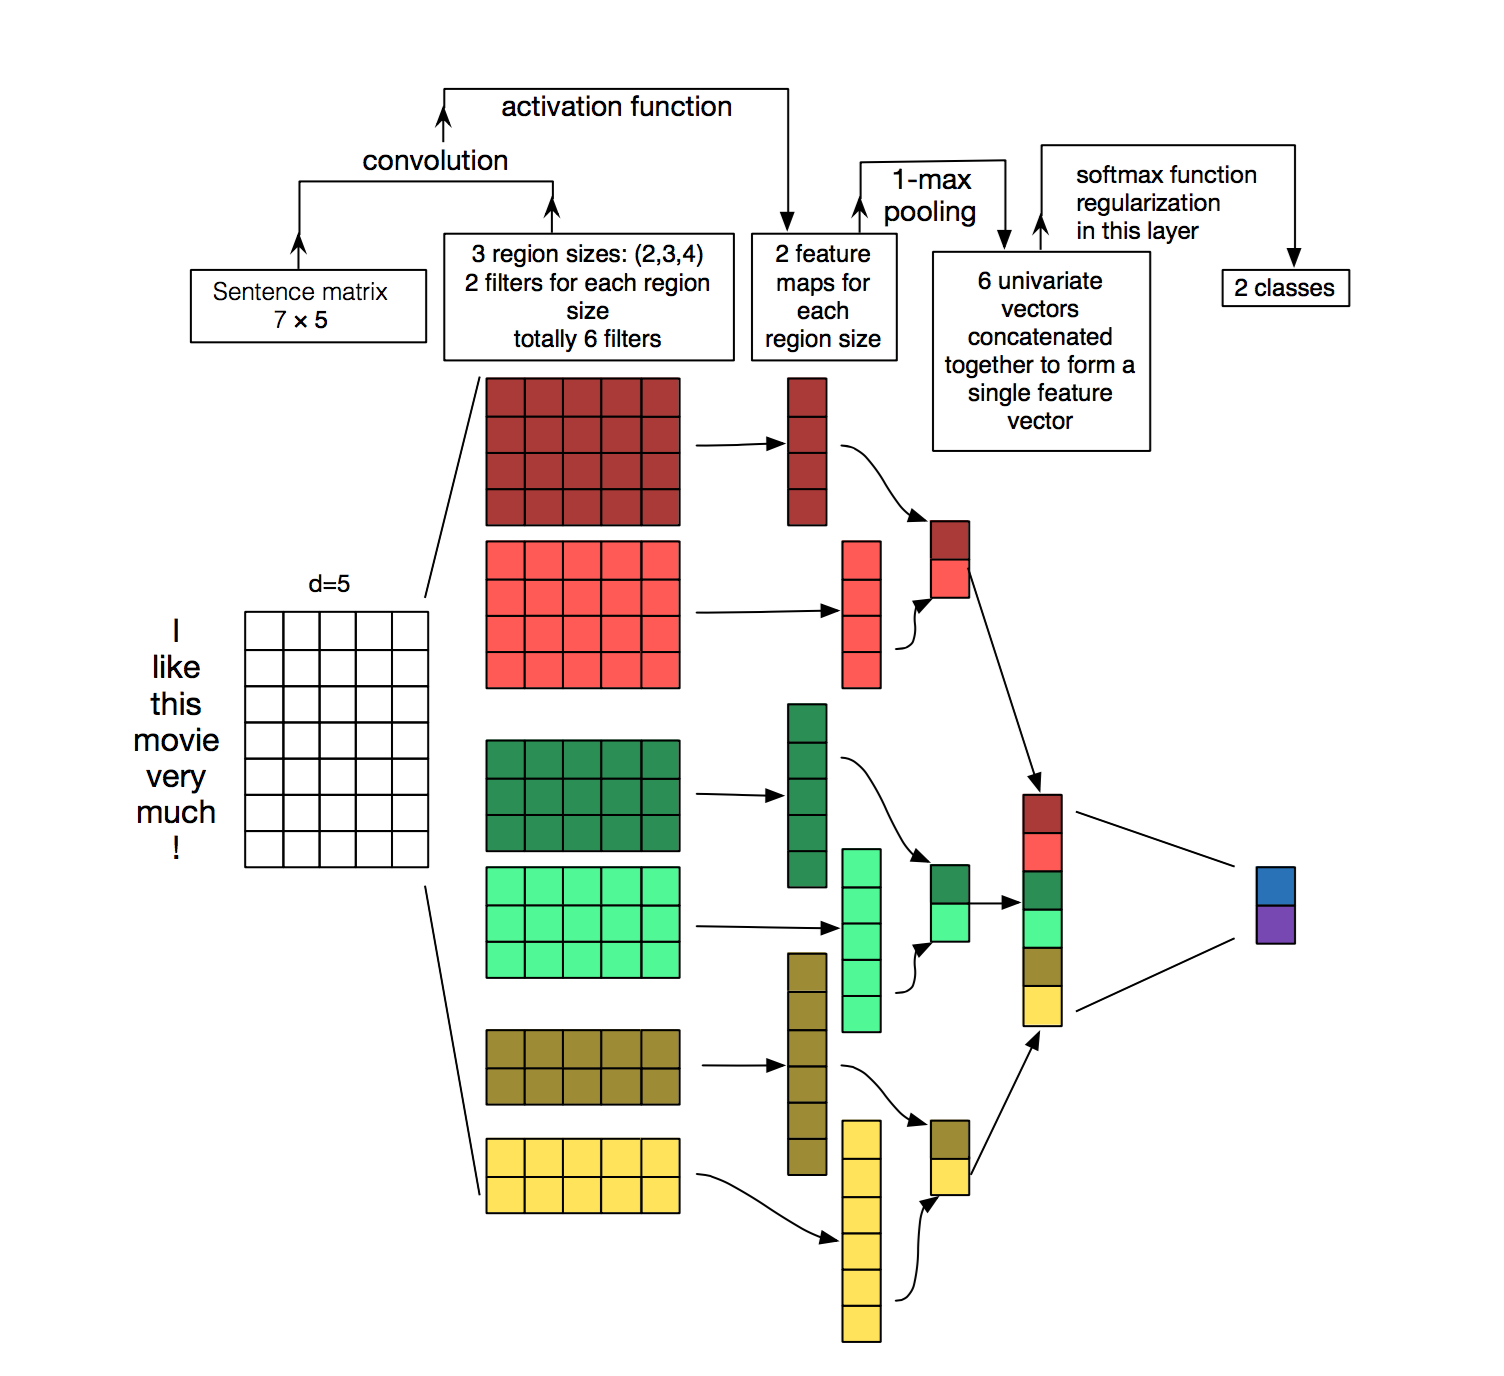
\includegraphics[width=\linewidth]{plots/multi-channel-CNN-architecture.png}
\caption{CNN Architecture}
\label{fig:architectureCNN}
\end{figure}

\begin{figure}[H]
\centering
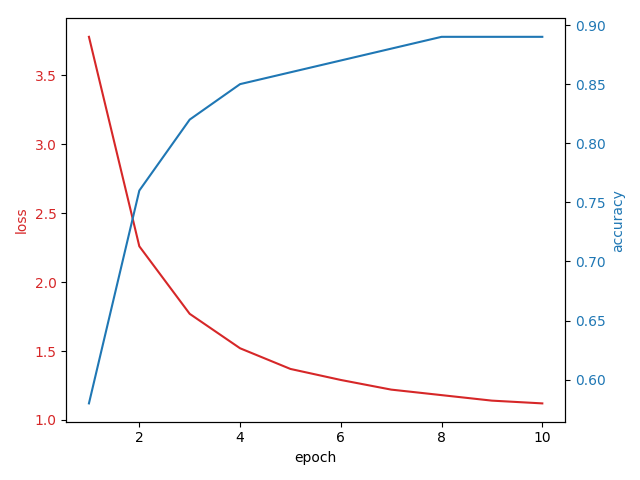
\includegraphics[width=\linewidth]{plots/learning_curve_cnn.png}
\caption{Learning Curve for CNN}
\label{fig:learningCurveCNN}
\end{figure}

\subsection{Performance Comparison}

We can see from the following Table~\ref{table:performanceComparison} that Precision@1 for CNN is only 0.56. This is most likely because the model is not able to accurately predict the class label. On the other hand, CNN performs much better for Precision@5 with an accuracy of 0.89.

Another interesting observation is that the Precision@5 accuracy for all the models caps out at 0.89. We think this is due to some underlying property or limitation of the dataset and requires further experimentation.

\begin{table}[H]
\begin{tabular}{|l|l|l|l|}
\hline
    & Precision@1 & Precision@3 & Precision@5 \\ \hline
NBC & 0.74        & 0.86        & 0.89        \\ \hline
LR  & 0.71        & 0.84        & 0.89       \\ \hline
CNN & 0.56        & -           & 0.89        \\ \hline
\end{tabular}
\caption{Precision@1, 3 and 5 for each Model}
\label{table:performanceComparison}
\end{table}

\section{Further Experiments}
\subsection{Toggle Title and Body}

Table~\ref{table:titleBodyToggled} shows the Precision@5 accuracy for both NBC and LR with only the posts' titles, only the posts' bodies and finally, with both.

The median length of the titles is 35 characters and 7 words. It is interesting to see that, even with such a small size, we can still distinguish between 1000 labels and get an accuracy of 0.59 and 0.64. This is pretty remarkable and can lead to further research on similar problems.

However, we also find that, given the body, the title alone does not add too much information and we do not see much increase in the accuracies of the models. This confirms our earlier intuition that the content of the title and the body are similar for a post and are very closely related to the subreddit that it was posted in.

\begin{table}[H]
\begin{tabular}{|l|l|l|}
\hline
           & Naive Bayes Classifier & Logistic Regression \\ \hline
Title Only & 0.64                   & 0.59                \\ \hline
Body Only  & 0.87                   & 0.86                \\ \hline
Both       & 0.89                   & 0.89                \\ \hline
\end{tabular}
\caption{Precision@5 with Title and Body Toggled}
\label{table:titleBodyToggled}
\end{table}

\subsection{Feature Importance Analysis}

Figures ~\ref{fig:featureImportanceGOT}-~\ref{fig:featureImportanceCricket} show the feature importance for three subreddits: r/gameofthrones, r/rickandmorty, and r/cricket. Note that these were obtanied from stemmed data, so the graphs only show stemmed features.

We can see from these figures that our model seems to capture the key features of the respective subreddits. For example, "king", "dragon", "north" are of high importance in r/gameofthrones (Figure \ref{fig:featureImportanceGOT}); "rick", "portal", "federation" are of high importance in r/rickandmorty (Figure \ref{fig:featureImportanceRickAndMorty}); and "cricket", "match", "bat" are of high importance in r/cricket (Figure \ref{fig:featureImportanceCricket}).

However, we can also see that some features were mistakenly given high importance. For example, "http" was given a high importance in r/cricket, which does not really make sense. This suggests scope for improvement in future work.

\begin{figure}[H]
\centering
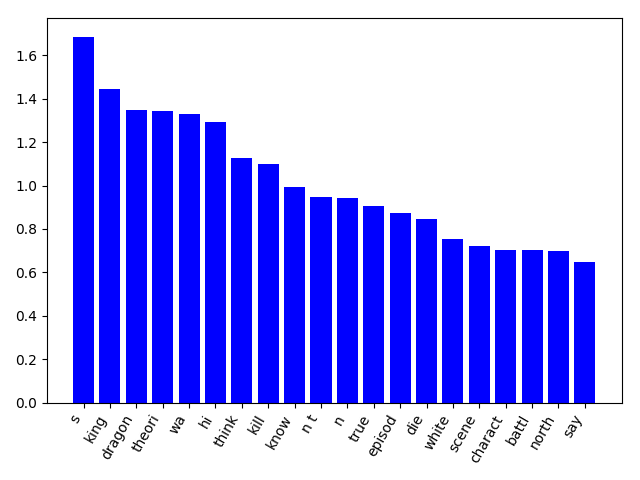
\includegraphics[width=\linewidth]{plots/coefficients-gameofthrones-dim-337.png}
\caption{Important Features for subreddit r/gameofthrones}
\label{fig:featureImportanceGOT}
\end{figure}

\begin{figure}[H]
\centering
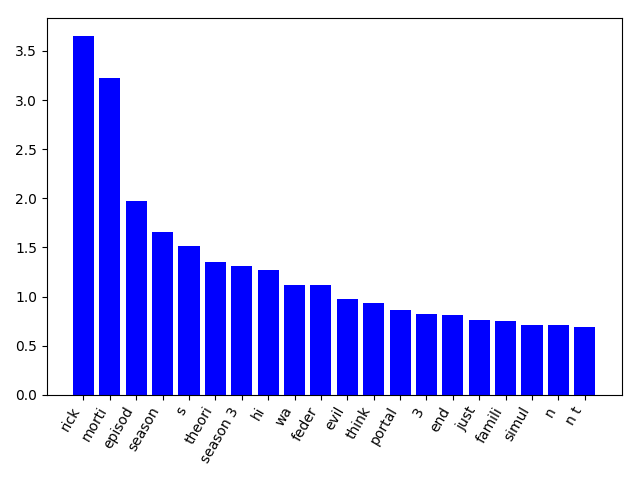
\includegraphics[width=\linewidth]{plots/coefficients-rickandmorty-dim-713.png}
\caption{Important Features for subreddit r/rickandmorty}
\label{fig:featureImportanceRickAndMorty}
\end{figure}

\begin{figure}[H]
\centering
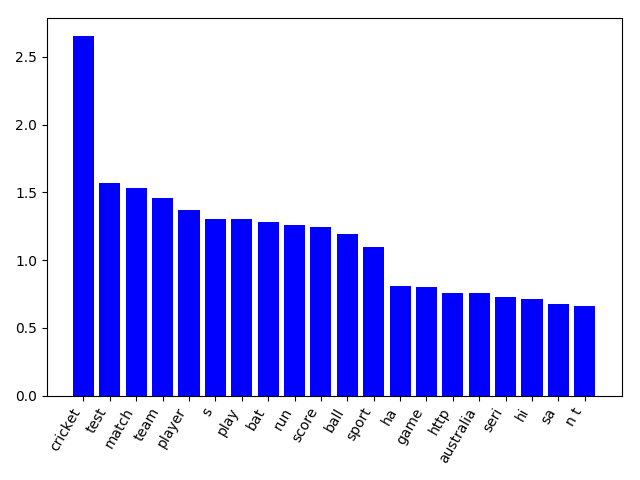
\includegraphics[width=\linewidth]{plots/coefficients-cricket-dim-200.png}
\caption{Important Features for subreddit r/cricket}
\label{fig:featureImportanceCricket}
\end{figure}

\subsection{Performance Using Features for Sentiment Analysis and Readability Level}

We used Python's \verb+TextBlob+\cite{textblob} library to get the sentiment value of each post. Similarly, we used Python's \verb+textstat+\cite{textstat} library to compute the readability score of each post.

We compared the behaviour of Logistic Regression with and without those features on 100k rows of the dataset:

\begin{table}[H]
\begin{tabular}{|l|l|l|l|}
\hline
    & Prec@1 & Prec@3 & Prec@5 \\ \hline
With sentiment and readability & 0.01        & 0.02        & 0.02        \\ \hline
Without those features  & 0.58        & 0.75        & 0.80       \\ \hline
\end{tabular}
\caption{Sentiment and readability level: Precision}
\label{table:sentiment}
\end{table}

Unfortunately, adding those two features degrades performance completely. We believe it is because we add those two features to the sparse matrix that we get after vectorizing the bag-of-words, which leads the model to overweight those features even when they are not highly informative. In any case, we report our experimental results above.

\subsection{Confusion Matrix}

To analyze which subreddits are frequently mispredicted, we look at the confusion matrix. As the 1000x1000 matrix for all the labels was hard to read, we have zoomed in on the subreddits that were most frequently confused.

Figure \ref{fig:confusionMatrix1} shows the top 40 most-confused subreddits, where we can see the characteristic diagonal of dark squares along with a few lighter squares denoting the mispredicted labels.

\begin{figure}[H]
\centering
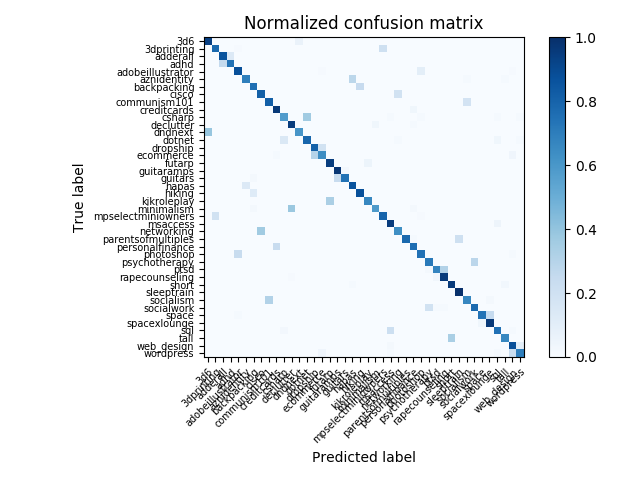
\includegraphics[width=\linewidth]{plots/confusion-matrix-top-confused-labels-all.png}
\caption{Confusion Matrix of the Top-40 Most-Confused Subreddits}
\label{fig:confusionMatrix1}
\end{figure}

Another version is in Figure \ref{fig:confusionMatrix2} where we can see that r/Adderall and r/ADHD are often confused, as are r/dropship and r/ecommerce.

\begin{figure}[H]
\centering
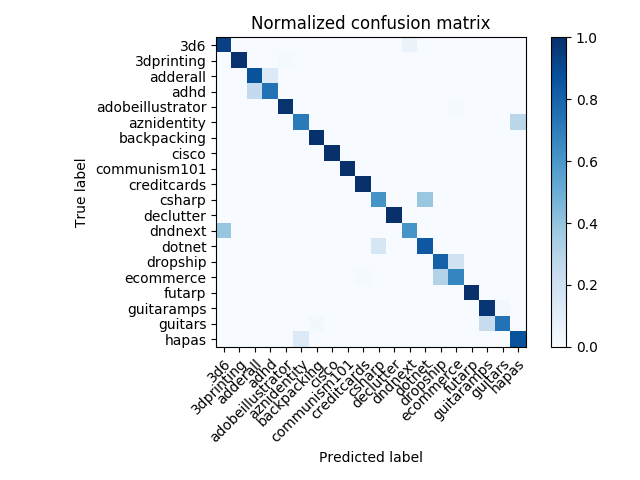
\includegraphics[width=\linewidth]{plots/confusion-matrix-top-confused-labels-0-to-20.png}
\caption{Another Version of the Confusion Matrix}
\label{fig:confusionMatrix2}
\end{figure}

Again, since the matrix is quite sparse it is hard to show them on the same plot, so we decided to visualize the true label along with its most-confused label in the same plot (Figure \ref{fig:confusionMatrix3}). We see that posts from r/hiking are attributed to r/backpacking, posts from r/cisco are attributed to r/networking, and, for some reason, posts from r/short are attributed to r/tall (probably because both talk about height).

\begin{figure}[H]
\centering
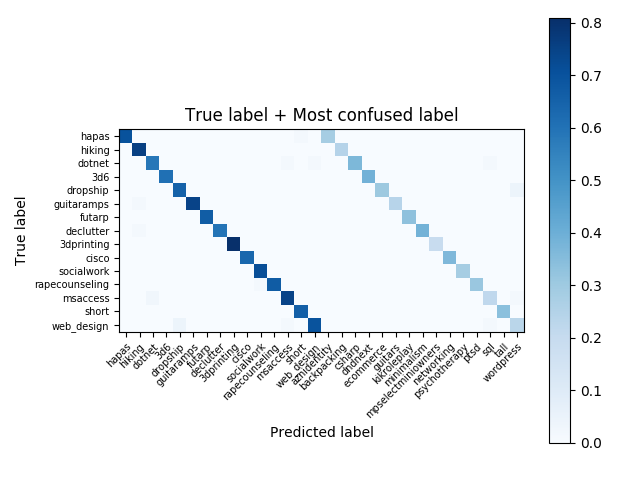
\includegraphics[width=\linewidth]{plots/confusion-matrix-true-label-vs-most-confused-label.png}
\caption{True Label and Most-Confused Label on Same Graph}
\label{fig:confusionMatrix3}
\end{figure}

To get a better idea of what confuses the model, we look at two concrete subreddits: r/hiking and r/backpacking:

\begin{figure}[H]
\centering
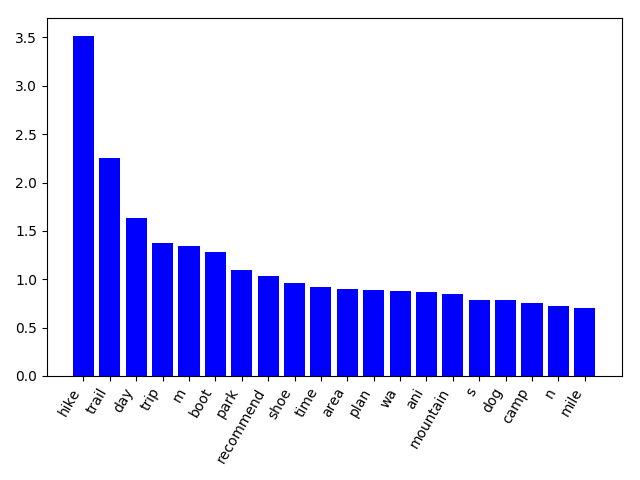
\includegraphics[width=\linewidth]{plots/coefficients-hiking-dim-393.png}
\caption{Important Features for subreddit r/hiking}
\label{fig:featureImportanceHiking}
\end{figure}

\begin{figure}[H]
\centering
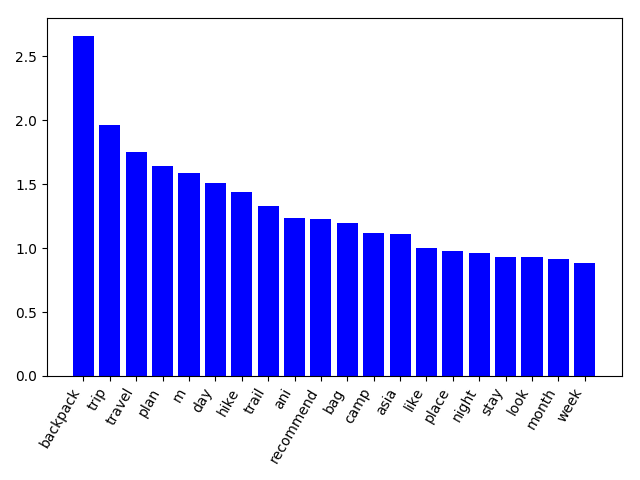
\includegraphics[width=\linewidth]{plots/coefficients-backpacking-dim-78.png}
\caption{Important Features for subreddit r/backpacking}
\label{fig:featureImportanceBackpacking}
\end{figure}

If we compare their most important features (Figure \ref{fig:featureImportanceHiking} and Figure \ref{fig:featureImportanceBackpacking}), we find that many of them are the same, such as ``trip'', ``day'', ``plan'', ``trail'', and ``camp''. This might be an inherent limitation of the dataset, because these are not well-separated subreddits and we may not be able to distinguish them given the posts alone.

\section{Evaluation of Project Goals}

Our project goals consisted of:
\begin{enumerate}
    \item Preprocessing

            We preprocessed the data by converting it to lowercase, removing encoded HTML and other tags, removing punctuations and stemming the words.
    \item Exploratory Data Analysis

            Exploratory Data Analysis was done by exploring the sample distribution length for the title and body of the posts and by plotting a TSNE plot to see if similar subreddits are clustered together.
    \item Implementing algorithms

            We implemented two traditional learning algorithms (Naive Bayes Classifier and Logistic Regression) and a deep learning model (Convolutional Neural Network). We also tuned the hyper parameters of these algorithms to get the best possible performance on our dataset.
    \item Experiment with adding new features

            In order to see if we can extract even more information from the data, we added features for the sentiment value and readability score of every post in the dataset.
    \item Toggling post's title and body

            To understand the impact of the title on classification, we measured the performance by training and testing on just the titles of the posts, just the bodies of the posts, and then with both title and body.

\end{enumerate}

In addition to the above, we also computed the confusion matrix and carried out qualitative analysis by computing the feature importance for our models.

We, therefore, have achieved our goals that we set in the project proposal.

\section{Conclusions}

Overall, we were able to get good results on the RSPCT dataset, which supports our hypothesis that one of the main bottlenecks in large text classification tasks is the sparsity of examples for labels. All three models were clearly able to learn over the dataset and curiously produced very similar results for the top-5 classification accuracy. Future work might focus on either increasing the accuracy on this dataset using better model and more tuning or aggregating such a large number of examples per label for other tasks (perhaps using Reddit itself). Another question to answer is whether adding more than 1000 examples per label might improve accuracy even further or whether the benefits would taper off.

Our experiments on the title and body showed us that as few as 7 words could allow a reasonably-high degree of accuracy even with 1000 labels. Our investigation of the feature importance shows us the strengths of the models and points to clear steps for future work. Finally, our analysis of the confusion matrix points to the most-confused subreddits, which could inform future work in this area.

\section{Acknowledgements}

We would like to thank Professor Ming Yin for her suggestion about using a confusion matrix for pinpointing the subreddits that frequently confused our model.

\section{Team Member Contributions}

Pradeep Kumar Srinivasan: Worked on model implementation and tuning, report, confusion matrix, presentation, slides, feature importance

Mohammad Haseeb: Worked on preprocessing, exploratory data analyis, sentiment value and readability score features, slides, presentation, report

%\end{document}  % This is where a 'short' article might terminate

%
% The following two commands are all you need in the
% initial runs of your .tex file to
% produce the bibliography for the citations in your paper.
\bibliographystyle{abbrv}
\bibliography{sigproc}  % sigproc.bib is the name of the Bibliography in this case
% You must have a proper ".bib" file
%  and remember to run:
% latex bibtex latex latex
% to resolve all references
%
% ACM needs 'a single self-contained file'!
%% \subsection{References}

\end{document}

%%% Local Variables:
%%% mode: latex
%%% TeX-master: t
%%% End:
